\documentclass{article}
\usepackage{graphicx} % Add this line here
\usepackage{amsmath}
\usepackage{xcolor} % Add this line before \usepackage{mdframed}
\usepackage{mdframed}
\usepackage{float}
\usepackage{longtable}
\usepackage{tikz}
\tikzstyle{bag} = [text width=4em, text centered]

\title{Climate Risks}
\author{Thomas Lorans}
\date{\today}

\begin{document}

\maketitle

\begin{abstract}
 
\end{abstract}


\section{Investment Under Uncertainty}

\subsection{Two-Period Model}

A firm is considering investing 
in a widget factory. The investment 
cost $I$ is 1600 USD. 
Currently, price of a widget is 200 USD, but next year the price will change.
With probability $q$, it rises to 300 USD and with probability $1-q$ it falls to 100 USD.
The risk-free rate is 10\% and is used as the discount rate.


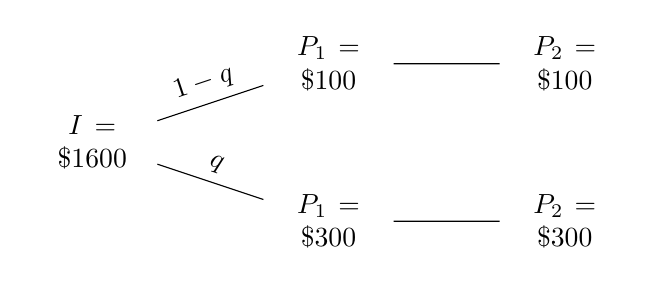
\begin{tikzpicture}[grow=right, sloped, 
    level distance=3cm, % Adjusts the distance between levels
    sibling distance=2cm] % Adjusts the distance between siblings
    \node[bag] {$I = \$1600$}
    child {
        node[bag] {$P_1 = \$300$}        
            child {
                node[bag] {$P_2 = \$300$}        
                edge from parent 
                node[above] {}
            }
            edge from parent 
            node[above] {$q$}
    }
    child {
        node[bag] {$P_1 = \$100$}
            child {
                node[bag] {$P_2 = \$100$}        
                edge from parent 
                node[above] {}
            }   
            edge from parent
            node[above] {$1-q$}
    };
\end{tikzpicture}

The Net Present Value (NPV) of the investment is given by:

\begin{equation}
    NPV = - I + \sum^{\infty}_{t=0} \frac{E[P]}{1 + r}^t
\end{equation}

where $E[P]$ is the expected price of a widget in the future and $r$ is the discount rate.
The expected price of a widget in the future is given by:

\begin{equation}
    E[P] = q \cdot 300 + (1-q) \cdot 100
\end{equation}

We obtain a value of $E[P] = 200$ USD.
$\sum^{\infty}_{t=0} \frac{200}{1.1^t}$ is a geometric series that converges to 2200
Replacing with our numerical values, we get:

\begin{equation}
    \sum^{\infty}_{t=0} \frac{200}{1.1^t} = \frac{200}{1 - \frac{1}{1.1}} \approx 2200
\end{equation}

Plugging this into the NPV formula, we get:
\begin{equation}
    NPV = -1600 + \sum^{\infty}_{t=0} \frac{200}{1.1^t} = -1600 + 2200 = 600
\end{equation}

It seems that the investment is profitable, 
as the current value of the investment, $V_0$, is equal to 2200 USD
and exceeds the initial cost $I$ of 1600 USD.

\section{Adaptation in Face of Climate Change}

\section{Green Investment in Face of Transition}

% \subsection{Industrials Case Study: Application to xxxx}

% \subsection{Transport Case Study: Application to xxxx}

% \subsection{Oil, Gas \& Consumable Fuels Case Study: Application to xxxx}

% \subsection{Agriculture Case Study: Application to xxxx}


\newpage
\bibliographystyle{plain} % This defines how bibliography entries are formatted.
\bibliography{refs} % This includes the bibliography in your document.

\end{document}
